\chapter{From Technical Fluency to Operating Scope}

We begin with a question about transfer. A student of computer science appears first as a programmer, and yet the career described here ends in operating leadership, healthcare technology, and a company sold for \$3.5 billion. The lecture does not answer this by abstraction alone. It proceeds in order: programming, devices, protocols, people, field work, consulting, and finally executive scope. The mathematics in these notes is therefore schematic rather than literal. It serves to preserve the monotone growth of responsibility that the speaker narrates.

\section{The Opening Transfer Question}

The opening prompt contains two questions at once. How does computer science lead to the present role, and are the early technical skills still useful later on? We should keep both parts in view, because the lecture answers them together.

A compact way to state the initial puzzle is
\begin{equation}
\text{computer science} \;\to\; \text{current executive role},
\end{equation}
together with the related question
\begin{equation}
\text{early technical skills} \;\to\; \text{later operating usefulness}.
\end{equation}
What matters in the rest of the lecture is that neither arrow is treated as mysterious. The speaker fills in the intermediate stages one by one.

\section{Starting Point: Programmer and Devices}

The first answer is deliberately narrow: the speaker started as a computer programmer. That starting point matters because it prevents the later career from being read backward as if executive authority had been there from the beginning.

From there the first expansion is not yet managerial. It is still technical, but technical work now touches real devices in real environments:
\begin{equation}
\text{computer programmer} \;\to\; \text{device programming}.
\end{equation}
The named examples, B-1 bombers and Disneyland, are important less for glamour than for scale and concreteness. They tell us that the work was not merely symbolic manipulation on a screen. It involved machines, interfaces, and deployment conditions.

We may summarize the early sequence as
\begin{equation}
\text{computer programmer}
\;\to\;
\text{program all sorts of devices}
\;\to\;
\text{work in the field}.
\end{equation}
The lecture then pivots away from examples themselves and toward the lesson extracted from them.

\section{Protocols as the First Portable Abstraction}

The key sentence in the lecture is the move from devices to communication between devices. Once we are told that a box could be taken out to a device so that devices could talk to each other, the local programming task opens into a more general structure:
\begin{equation}
\text{device programming}
\;\to\;
\text{devices talk to each other}
\;\to\;
\text{protocols}.
\end{equation}
This is the first genuine abstraction in the story. The speaker is no longer naming projects. He is naming the mechanism that makes skills transferable.

We may then continue the same chain:
\begin{equation}
\text{protocols}
\;\to\;
\text{working with companies and people}.
\end{equation}

\begin{definition}
For the purposes of these notes, \emph{transferability} means that a skill learned at one scale of work can be carried to a broader scale without being discarded. In this lecture the speaker's transferable core is not only coding, but also protocol knowledge and coordination with companies and people.
\end{definition}

To keep the internal logic clear, let us introduce a schematic notation:
\begin{align}
T &= \text{technical fluency}, \\
F &= \text{field exposure}, \\
P &= \text{protocol knowledge}, \\
C &= \text{coordination with companies and people}.
\end{align}
Then the lecture's mechanism may be written, cautiously, as
\begin{equation}
S_{\text{scope}} = f(T,F,P,C),
\end{equation}
where \(S_{\text{scope}}\) denotes the scale of responsibility. This formula is not spoken in the lecture; it is a compact reconstruction of the lecture's logic.

\paragraph{A worked schematic derivation.}
We can now write the progression in short steps:
\begin{align}
(T,F) &\to \text{real device problems}, \\
\text{real device problems} &\to P, \\
P &\to C, \\
(T,F,P,C) &\to \uparrow S_{\text{scope}}.
\end{align}
The point is simple. Once a technical worker learns how systems interact, the work is no longer only about code. It becomes about interfaces, coordination, and eventually the organizations that must make those interfaces function.

\subsection{Question \& Answer}

\paragraph{Question.}
How do early technical skills transfer upward into an executive career, rather than remaining trapped at the level of programming?

\paragraph{Answer.}
The lecture's answer is that technical work becomes durable when it passes through protocols. A programmer who only writes code for isolated tasks remains local. A programmer who learns how devices communicate acquires protocol knowledge, and protocol knowledge immediately places one in contact with companies, people, and concrete field problems. It is at that point that technical fluency begins to widen into operating judgment.

\section{Field Work as the Career Hinge}

The next transition is motivational rather than purely technical. The speaker says he loved being in the field. We should not treat this as incidental autobiography. It is the hinge on which the rest of the career turns.

If we want a compact progression, we may write
\begin{equation}
\text{protocols}
\;\to\;
\text{field problem-solving}
\;\to\;
\text{career direction}.
\end{equation}
The lecture is saying that competence alone is not enough. Preference matters. The speaker does not merely know how to solve field problems; he likes doing so, and that taste directs the next move.

A useful schematic update rule is
\begin{equation}
S_{n+1} = \Phi(S_n),
\end{equation}
where \(\Phi\) means: take the skill at one scale and express it at the next larger scale of responsibility. In the present lecture we may read the first few iterates as
\begin{align}
S_0 &= \text{programmer}, \\
S_1 &= \text{device programmer}, \\
S_2 &= \text{inter-device problem solver}, \\
S_3 &= \text{field problem solver}.
\end{align}
Again, this is a bookkeeping device for the lecture's progression, not a formula claimed by the speaker.

\begin{figure}
\centering
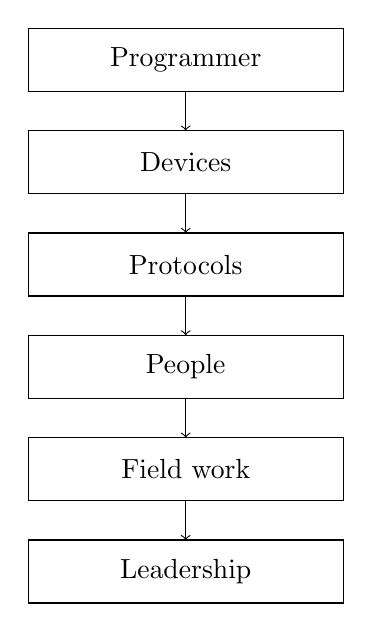
\begin{tikzpicture}[x=1cm,y=1cm]
\draw (0,0) rectangle (4,0.8);
\node at (2,0.4) {Programmer};

\draw[->] (2,0) -- (2,-0.5);

\draw (0,-1.3) rectangle (4,-0.5);
\node at (2,-0.9) {Devices};

\draw[->] (2,-1.3) -- (2,-1.8);

\draw (0,-2.6) rectangle (4,-1.8);
\node at (2,-2.2) {Protocols};

\draw[->] (2,-2.6) -- (2,-3.1);

\draw (0,-3.9) rectangle (4,-3.1);
\node at (2,-3.5) {People};

\draw[->] (2,-3.9) -- (2,-4.4);

\draw (0,-5.2) rectangle (4,-4.4);
\node at (2,-4.8) {Field work};

\draw[->] (2,-5.2) -- (2,-5.7);

\draw (0,-6.5) rectangle (4,-5.7);
\node at (2,-6.1) {Leadership};
\end{tikzpicture}
\end{figure}

The diagram is deliberately narrow. It shows that the lecture is built as a vertical expansion of scope, not as a sideways collection of unrelated experiences.

\section{From Field Problems to Institutional Scale}

From field work the lecture moves into institutions. Solving specific problems with people in the field leads, in the speaker's account, to Arthur Anderson, where he was a partner. We keep the transcript's wording here, while noting that the corporate spelling may require later verification.

The significant point is the pattern of enlargement:
\begin{equation}
\text{field problem-solving}
\;\to\;
\text{partner}
\;\to\;
\text{healthcare technology leadership}.
\end{equation}
The lecture then adds another layer:
\begin{equation}
\text{healthcare technology leadership}
\;\to\;
\text{worldwide consulting leadership}.
\end{equation}
What we see is not a break with the earlier technical base. We see its enlargement. The same person who once made devices talk to each other now works at a scale where institutions, rather than machines alone, must be made to work together.

\begin{remark}
The phrase in the transcript about healthcare IBM consulting worldwide is compressed. In these notes we preserve the direction of the claim rather than a more precise title that the transcript does not securely supply.
\end{remark}

\section{Operating Leadership and the Business Payoff}

The lecture ends not with a new principle, but with a measured outcome. The speaker says that he ultimately became chief operating officer for HMS Holdings, a healthcare company that was sold for \$3.5 billion. The final number should be kept exactly, but also kept in its proper place: as the payoff to the preceding chain.

We may write
\begin{equation}
\text{worldwide consulting leadership}
\;\to\;
\text{COO at HMS Holdings}
\;\to\;
V_{\text{exit}},
\end{equation}
with
\begin{equation}
V_{\text{exit}} = \$3.5\,\text{billion}.
\end{equation}
This is not yet a valuation model, and the lecture does not try to make it one. The number functions as evidence that the long path from programming to operating responsibility can culminate in large-scale enterprise value.

If we compress the entire lecture into one final structural relation, we obtain
\begin{equation}
T + F + P + C \;\Longrightarrow\; \uparrow S_{\text{scope}} \;\Longrightarrow\; V_{\text{exit}}.
\end{equation}
That last equation is a reconstruction, but it captures the shape of the argument well: technical fluency survives, field exposure deepens it, protocol knowledge broadens it, coordination scales it, and the result is a much larger domain of responsibility.

\section{Summary}

The lecture's force comes from its refusal to leap. We do not jump from computer science to CEO. We pass through programming, devices, inter-device communication, protocols, companies and people, field work, consulting, institutional leadership, and only then to chief operating responsibility and a \$3.5 billion outcome.

That is the transferable lesson. Early technical skill matters, but it matters most when it teaches us how systems connect and how people coordinate around those connections. In that sense the lecture is not about leaving the technical world behind. It is about carrying its deepest structures upward into larger and larger forms of work.